\section{Suddivisione del lavoro}
I componenti del gruppo dovranno rivestire ogni ruolo almeno una volta. Possono ricoprire più ruoli contemporaneamente purché non si presentino conflitti di interesse tra i ruoli ricoperti.
	\subsection{Dettaglio Fasi}
		\subsubsection{Analisi}
		Nella fase di Analisi, ciascun componente dovrà ricoprire i seguenti ruoli: \\
		I valori sono riassunti nel seguente grafico, che rappresenta in maniera visiva per quante ore un membro abbia ricoperto un determinato ruolo.
		\begin{figure}[htbp]
			\centering
			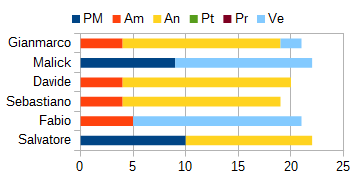
\includegraphics[scale=1]{immagini/grafici/analisi-barra.png}
			\caption{Ore per componente, fase di Analisi}
		\end{figure}
		\subsubsection{Analisi di Dettaglio}
		Nella fase di Analisi di Dettaglio, ciascun componente dovrà ricoprire i seguenti ruoli: \\
		I valori sono riassunti nel seguente grafico, che rappresenta in maniera visiva per quante ore un membro abbia ricoperto un determinato ruolo.
		\begin{figure}[htbp]
			\centering
			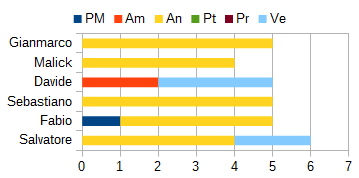
\includegraphics[scale=1]{immagini/grafici/analisi_dettaglio-barra.png}
			\caption{Ore per componente, fase di Analisi di Dettaglio}
		\end{figure}
		\subsubsection{Progettazione Architetturale}
		Nella fase di Progettazione Architetturale, ciascun componente dovrà ricoprire i seguenti ruoli: \\
		I valori sono riassunti nel seguente grafico, che rappresenta in maniera visiva per quante ore un membro abbia ricoperto un determinato ruolo.
		\begin{figure}[htbp]
			\centering
			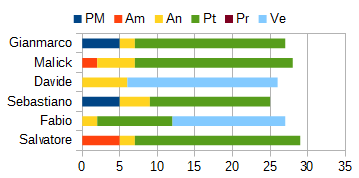
\includegraphics[scale=1]{immagini/grafici/progettazione_architetturale-barra.png}
			\caption{Ore per componente, fase di Progettazione Architetturale}
		\end{figure}
		\subsubsection{Progettazione di Dettaglio e Codifica}
		Nella fase di Progettazione di Dettaglio e Codifica, ciascun componente dovrà ricoprire i seguenti ruoli: \\
		I valori sono riassunti nel seguente grafico, che rappresenta in maniera visiva per quante ore un membro abbia ricoperto un determinato ruolo.
		\begin{figure}[htbp]
			\centering
			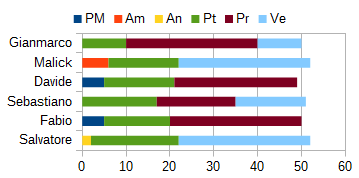
\includegraphics[scale=1]{immagini/grafici/progettazione_dettaglio_codifica-barra.png}
			\caption{Ore per componente, fase di Progettazione di Dettaglio e Codifica}
		\end{figure}
		\subsubsection{Verifica e Validazione}
		Nella fase di Verifica e Validazione, ciascun componente dovrà ricoprire i seguenti ruoli: \\
		I valori sono riassunti nel seguente grafico, che rappresenta in maniera visiva per quante ore un membro abbia ricoperto un determinato ruolo.
		\begin{figure}[htbp]
			\centering
			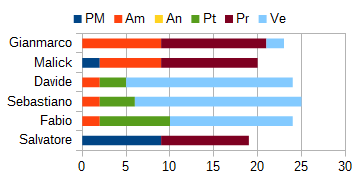
\includegraphics[scale=1]{immagini/grafici/validazione-barra.png}
			\caption{Ore per componente, fase di Verifica e Validazione}
		\end{figure}
	\subsection{Totali}
		\subsubsection{Ore totali con investimento}
		Le ore totali, comprese quelle di investimento, dedicate da ciascun componente all'intero progetto saranno le seguenti: \\
		I valori sono riassunti nel seguente grafico, che rappresenta in maniera visiva per quante ore un membro abbia ricoperto un determinato ruolo.
		\begin{figure}[htbp]
			\centering
			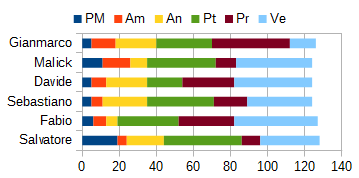
\includegraphics[scale=1]{immagini/grafici/riepilogo_conclusivo-barra.png}
			\caption{Ore per componente totali con investimento}
		\end{figure}
		\subsubsection{Ore rendicontate}